\section{\os 评估}
\label{s:eval}

\begin{figure*}[t]
  \centering
  \begin{minipage}[t]{0.31\linewidth}
    \centering
    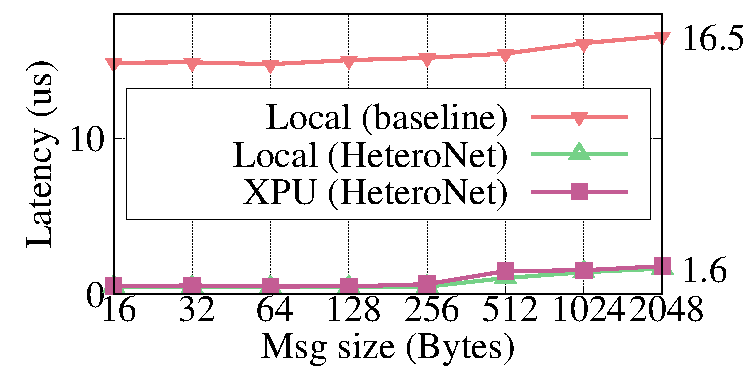
\includegraphics[width=0.98\linewidth]{figs-eval/eval-micro-socket-lat-eps-converted-to.pdf}\\[-0.5ex]
    \footnotesize\textbf{（a）延迟（小消息）。}
  \end{minipage}
  \begin{minipage}[t]{0.31\linewidth}
    \centering
    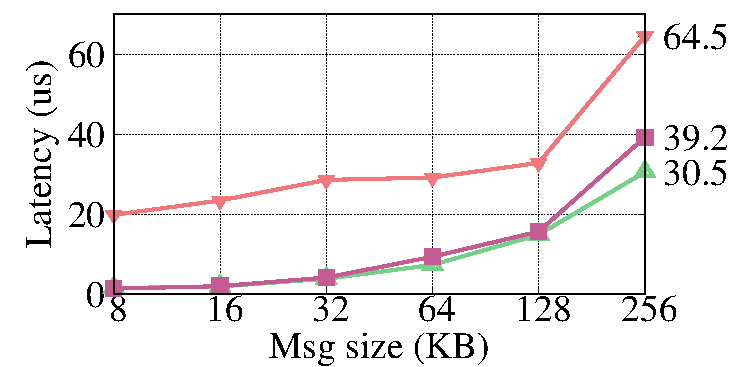
\includegraphics[width=0.98\linewidth]{figs-eval/eval-micro-socket-lat-large-eps-converted-to.pdf}\\[-0.5ex]
    \footnotesize\textbf{（b）延迟（大消息）。}
  \end{minipage}
  \begin{minipage}[t]{0.31\linewidth}
    \centering
    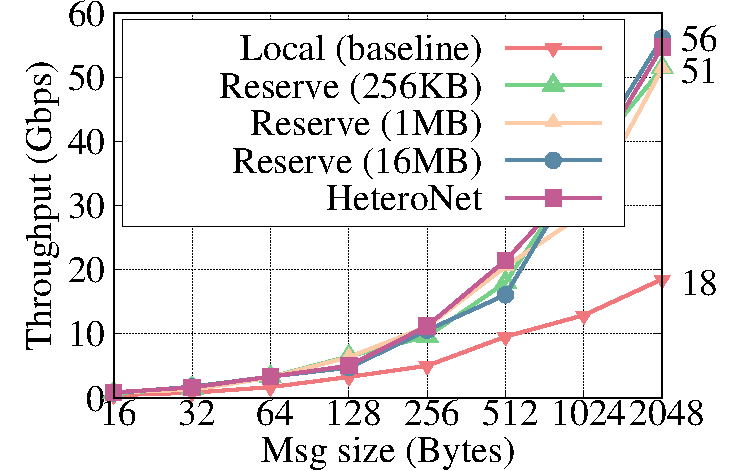
\includegraphics[width=0.98\linewidth]{figs-eval/eval-micro-socket-thr-eps-converted-to.pdf}\\[-0.5ex]
    \footnotesize\textbf{（c）吞吐量（Shm，小）。}
  \end{minipage}

  \begin{minipage}[t]{0.31\linewidth}
    \centering
    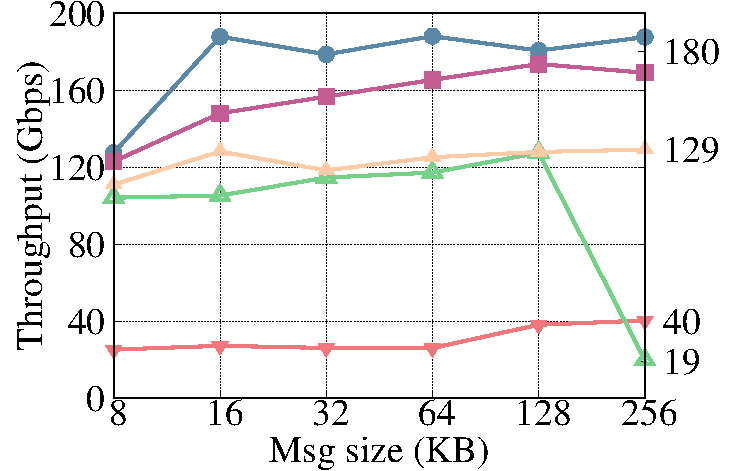
\includegraphics[width=0.98\linewidth]{figs-eval/eval-micro-socket-thr-large-eps-converted-to.pdf}\\[-0.5ex]
    \footnotesize\textbf{（d）吞吐量（Shm，大）。}
  \end{minipage}
  \begin{minipage}[t]{0.31\linewidth}
    \centering
    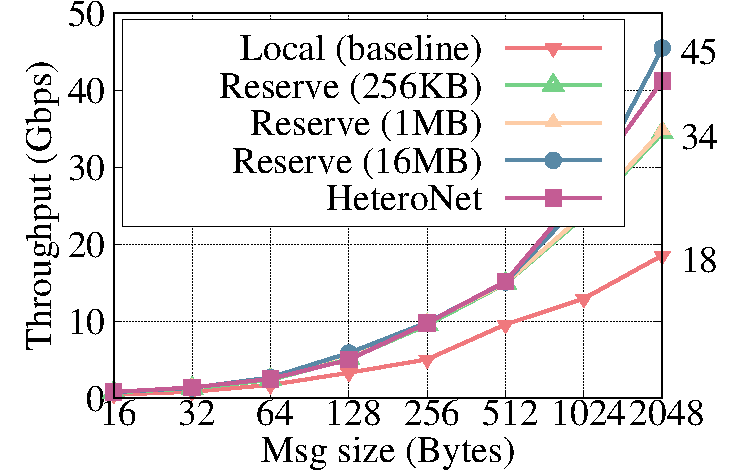
\includegraphics[width=0.98\linewidth]{figs-eval/eval-micro-socket-thr-cxl-eps-converted-to.pdf}\\[-0.5ex]
    \footnotesize\textbf{（e）吞吐量（CXL，小）。}
  \end{minipage}
  \begin{minipage}[t]{0.31\linewidth}
    \centering
    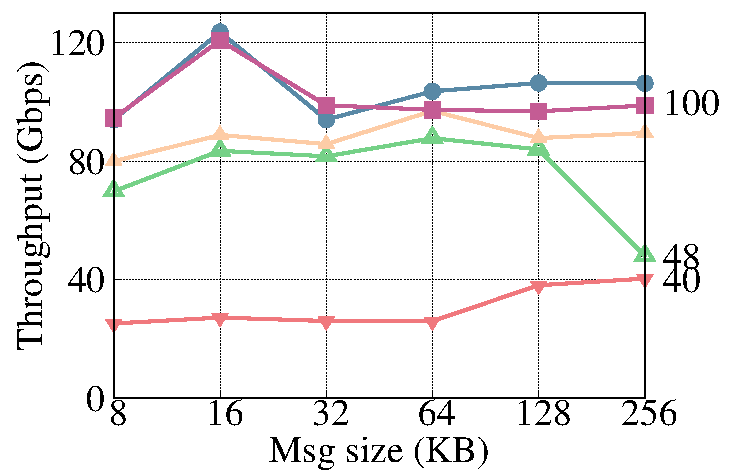
\includegraphics[width=0.98\linewidth]{figs-eval/eval-micro-socket-thr-large-cxl-eps-converted-to.pdf}\\[-0.5ex]
    \footnotesize\textbf{（f）吞吐量（CXL，大）。}
  \end{minipage}
  \caption{网络性能。}
  \label{fig:heterosocket-micro}
\end{figure*}

\subsection{\gsocket 性能}
\label{subs:eval-socket-microbench}

我们评估 \gsocket 的网络性能。测试使用 LMBench\cite{mcvoy1996lmbench}中的 \codeword{lat\_tcp} 和 \codeword{bw\_tcp}，分别测量网络延迟和吞吐量，并比较三种系统：（1）Baseline，即单个 PU 上使用 Linux 网络时的性能；（2）Reserve，即为每条连接预留特定大小 GShm 的 \os 版本，例如 1MB 表示连接为两个方向各预留一个 1MB 缓冲区；（3）\os，为本地记录使用 128KB，为共享区域使用 128MB。

\myparagraph{延迟。}
图~\ref{fig:heterosocket-micro}(a)(b)给出基线与 \os 的延迟，其中本地通信使用共享内存，XPU 通信使用 CXL。对于同一 PU 内的小消息，\os 相较基线将延迟降低 $10.1\times$（2KB）到 $31.9\times$（16B）；对于大消息，降低 $2.1\times$（256KB）到 $13.2\times$（8KB）。对于跨 PU 情形，基于 CXL 的 \os 可达到与共享内存相当的延迟，并比跨 PU 网络基线低两个数量级（因篇幅未在图中展示）。使用 CXL 时，U-NAPI 的一次跨 PU 通知约耗时 $0.51\,\mu$s，此外还需处理异常与上调的开销。

\myparagraph{吞吐量。}
图~\ref{fig:heterosocket-micro}(c)(d)给出 PU 内吞吐量，其中 \os 使用共享内存；图~\ref{fig:heterosocket-micro}(e)(f)给出跨 PU 吞吐量，其中 \os 使用 CXL。由于跨 PU 网络慢得多，基线仍使用 PU 内结果。图中还给出采用固定预留缓冲区、而不是本地记录与共享区域设计的 \os 结果。与基线相比，单 PU 上 \os 对小消息的吞吐量提升 $1.9$--$2.9\times$，对大消息提升 $4.8$--$6.3\times$；跨 PU 的 CXL 版 \os 也比单 PU 基线高 $1.4$--$4.4\times$。

\myparagraph{资源成本。}
假设图~\ref{fig:heterosocket-micro}(c)--(f) 中存在 1,000 条连接。每条连接预留 16MB 将占用 16GB 固定通信资源，是不可忽视的负担。每条连接只用 1MB（总计 1GB）或 256KB（1,000 条连接共享总计 256MB）时，小消息仍可达到良好吞吐量，但消息尺寸变大后会显著变慢，例如 256KB 配置慢超过 $2\times$。\os 使用 128KB 私有记录和 128MB 共享区域（总计 256MB），性能却几乎与预留 16MB 相同，在该情形中节省 $64\times$ 内存。我们在真实云环境中的实践是为 RDMA 每条连接预留 1MB，并为传统 Linux TCP 再预留 1MB，因此这一改善十分显著。

\begin{table}[t]
  \centering
  \footnotesize
  \caption{受支持应用的代码行数。\os 能支持代码规模显著更大的真实应用。\cmark 表示 Molecule 或 \os 支持，\xmark 表示不支持；CNN image 来自 FunctionBench，Alexa 来自 ServerlessBench。}
  \label{t:eval-efforts}
  \setlength{\tabcolsep}{3pt}
  \begin{tabular}{@{}lrrcc@{}}
    \toprule
    \textbf{应用} & \textbf{版本} & \textbf{LoC} & \textbf{Molecule} & \textbf{\os} \\
    \midrule
    Python3 & 3.8.10 & 1,085,262 & \xmark & \cmark \\
    Envoy & \#330dbdc8f9 & 764,457 & \xmark & \cmark \\
    \midrule
    CNN image & \#296f5f2 & 135 & \cmark & \cmark \\
    Alexa smarthome & \#207b345 & 1,804 & \cmark & \cmark \\
    \bottomrule
  \end{tabular}
\end{table}

\subsection{兼容性}

表~\ref{t:eval-efforts}比较 \sys 与 Molecule\cite{10.1145/3503222.3507732}所支持的两类最复杂应用的代码行数。Molecule 等框架虽然通过新抽象成功支持无服务器计算，却很难支持基于 Python 的服务和 Envoy\cite{envoy}等通用云原生应用；Envoy 在服务网格中被广泛采用。\sys 借助 \os，能够在 CPU--DPU 计算机上支持代码行数显著更高的通用应用，形成一个新的里程碑。

\myparagraph{支持其他异构设备。}
\os 可以推广到其他通用异构设备。但对于 FPGA、GPU 等领域专用加速器，应用通常不依赖套接字之类的 API；这时可以直接使用 DMA 等低级抽象进行高效通信。未来也可以结合 GPUnet\cite{kim2014gpunet}、Lynx\cite{tork2020lynx}和 Coyote\cite{korolija2020abstractions}等相关系统扩展 \os。

\myparagraph{支持其他系统。}
我们基于 Kubernetes 实现原型，因为它是目前使用最广泛的云原生平台\cite{cncf-landscape}。不过，动态拆分的思想以及 \giptable、\gsocket 两项技术具有通用性；实现也可以用于云原生应用之外的其他场景。

\myparagraph{局限。}
当前原型支持通过 libc 动态链接的应用使用 \gsocket，但不支持预先静态编译的应用；通过重新编译可以支持后者。\os 主要关注通过网络协作的应用。既有工作\cite{10.1145/3503222.3507732}已经支持 IPC 情形，未来将把该能力集成进来。线程等更细粒度的卸载仍是有待未来解决的开放问题。XPU 的更多策略和收益，例如能效\cite{234944}，也值得探索，但它们与本文所提供的动态拆分\emph{机制}相互正交。

\section{相关工作}
\label{s:relwk}

\myparagraph{异构计算机的系统支持。}
已有大量相关研究\cite{phothilimthana2018floem,seshadri2014willow,gu2016biscuit,baumann2009multikernel,barbalace2015popcorn,gamsa1999tornado,silberstein2013gpufs,kim2014gpunet,silberstein2017omnix,tork2020lynx,brokhman2019gaia,shan2018legoos,Asmussen:2016:MHC:2872362.2872371,nider2021last,pemberton2021restless,10.1145/3458336.3465273,liu2019offloading,cho2020flick}。分布式操作系统\cite{baumann2009multikernel,silberstein2017omnix,barbalace2015popcorn}使用包含多个内核的单一操作系统来管理异构设备。另一些系统使用智能设备卸载特定任务\cite{phothilimthana2018floem,seshadri2014willow,gu2016biscuit,kim2014gpunet,silberstein2013gpufs}。Floem\cite{phothilimthana2018floem}为 NIC 加速应用提出编程抽象；LeapIO\cite{li2020leapio}使用协处理器卸载云存储服务；E3\cite{234944}是面向 SmartNIC 加速服务器的微服务执行平台，可显著提高能效。作者认为，\os 是首个利用网络抽象实现动态拆分的系统；\sys 上的实践证明了该方法的可行性与效率。

\myparagraph{优化跨 PU 通信。}
既有工作\cite{10.1145/2934872.2934897,10.1145/2872362.2872401,10.1145/3230543.3230560,234944}已经探索利用 PCIe/DMA 高效实现 SmartNIC 与主机通信。GPUnet\cite{kim2014gpunet}为 GPU 程序提出套接字抽象；Solros\cite{min2018s}和 SPIN\cite{bergman2017spin}使用 P2P DMA 优化通信；Pond\cite{10.1145/3575693.3578835}利用 CXL 实现内存池化；CXL-Shm\cite{10.1145/3600006.3613135}利用 CXL 实现高效分布式共享内存，并以引用计数处理部分故障。作者认为，\os 是其中首个提供网络抽象的系统。

\myparagraph{相关网络方案。}
SocksDirect\cite{10.1145/3341302.3342071}提出用户空间套接字系统，使用用户态监控器管理资源与事件；但它并非针对 XPU 计算机，仍依赖预留内存缓冲区。SMC-R\cite{rfc7609}在内核中支持基于 RDMA 共享内存的网络，能够有效管理资源并支持商用应用，但以内核为中心的设计会产生用户态与内核态之间切换、复制的成本。IX\cite{belay2014ix}提出数据面操作系统，同时提供高 I/O 性能和保护。Arrakis\cite{peter2015arrakis}、mTCP\cite{10.5555/2616448.2616493}、F-stack\cite{f-stack}等同样保留 POSIX API 的内核旁路网络库，通常采用高效的用户空间 TCP/IP 实现和 DPDK。MegaPipe\cite{10.5555/2387880.2387894}与 StackMap\cite{196184}则使用零复制 API 优化网络栈。\os 延续这一研究方向，并提出推测式分配与 U-NAPI，在异构计算机中平衡性能和资源效率。

\section{结论}
\label{s:conclusion}

本文提出由 \os 支撑的 \xpod，使云原生应用能够在 CPU--DPU 计算机上进行动态拆分。\os 包含用于提供统一网络命名空间的 \giptable，以及同时取得内核旁路性能与内核辅助资源效率的 \gsocket。我们构建 \sys，并在无服务器计算和微服务等代表性云原生场景中展示其收益。作者计划开源 \os。
